\documentclass[12pt]{article}
\usepackage[utf8]{inputenc}
\usepackage[
    left=2.5cm,
    right=2.5cm,
    top=4cm,
    bottom=4cm
]{geometry}
\usepackage{courier}
\usepackage{listings}
\usepackage{tocloft}
\usepackage{xcolor}
\usepackage{amsmath}
\usepackage{mathtools}
\usepackage{amsfonts}
\usepackage{fancyhdr}
% \usepackage{palatino}

% \renewcommand{\familydefault}{\sfdefault}

\lstset{basicstyle=\footnotesize\ttfamily, breaklines=true, numbers=left, language=Python, tabsize=2, aboveskip=15pt, belowskip=15pt}

% Floor and Ceiling
\newcommand\floor[1]{\lfloor#1\rfloor}
\newcommand\ceil[1]{\lceil#1\rceil}

% Github style syntax highlighting
\newcommand{\highlight}{\colorbox{orange!60}}

% Does anyone like bullet points?
\def\labelitemi{--}

\setlength{\headheight}{15.0pt}
\pagestyle{fancy}
\lhead{6.046 Lecture 2: DNC}
\chead{Jing Lin. Kerberos: Jinglin}
\rhead{Nov. 12 2017}

\begin{document}
\section*{Median Finding Algorithms}
\par{There are a few approaches to finding the median of a list.  One approach is to sort the elements of the list and then compute the position of the median. That approach takes $\Theta(n \log{n})$ time.}
\par{Another approach inspired by quicksort is to find a pivot, and recurse on a subarray based on the rank of the pivot. The corresponding pseudocode is presented below.}

\begin{lstlisting}
	SELECT(S, i):
		Pick x in S cleverly
		Compute k = rank(x)
		B = Set of elements in S, such that elements < x
		C = Set of elements in S, such that elements > x
		if k == i:
			return x
		else if k > i:
			return SELECT(B, i)
		else if k < i:
			return SELECT(C, i - k)	
\end{lstlisting}

\par{The intuition here is if we can eliminate either B or C cleverly, and prove that the subarray we recurse on is always a fraction of the previous array, the algorithm will run in $\Theta(n)$ time.}

\begin{figure}[h]
	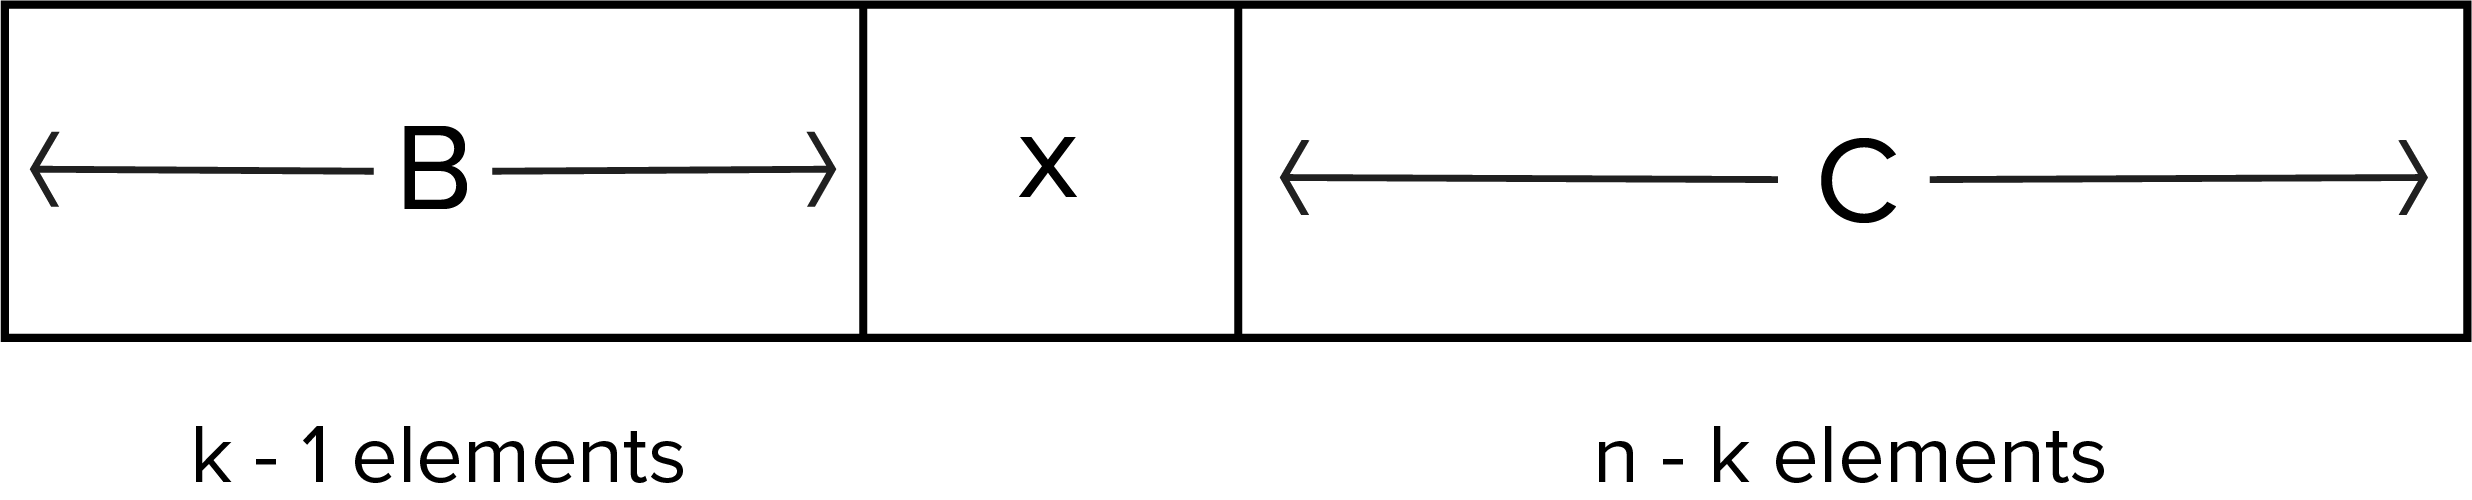
\includegraphics[width=0.7\textwidth]{../Illustrations/medians.png}
	\centering
\end{figure}

Without a clever strategy, if we’re selecting the $n - 1$ element and $k = 1$ every time, then we’re eliminating only one element on every iteration. There would be $n$ iterations, each taking $\Theta(n)$ time to partition the subarray. Therefore, the algorithm would run in $\Theta(n^2)$.

\subsubsection*{Clever Partitioning}
\begin{enumerate}
\item Arrange $S$ into columns of size 5 ($\ceil{n / 5}$ columns).
\item Sort each column in linear time (top down)
\item Find the medians of medians as $x$.
\end{enumerate}

\begin{figure}[h]
	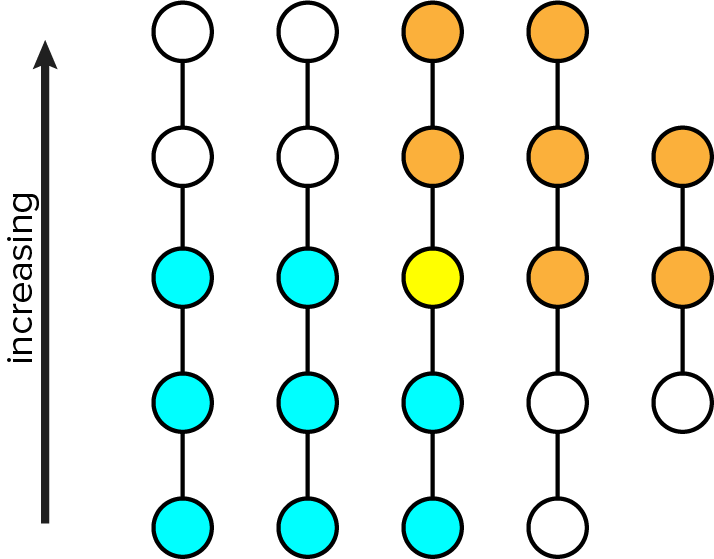
\includegraphics[width=0.5\textwidth]{../Illustrations/medians_circles.png}
	\centering
	\caption{The cyan circles are the elements lower than $x$ (denoted by the yellow circle) and the orange circles are the elements greater than $x$}
\end{figure}

\par{Half of the $\ceil{n / 5}$ groups contribute at least 3 elements $> x$ except for $1$ trailing group which could contain fewer than $5$ elements and $1$ group containing $x$. Therefore, there are at least $3(\ceil{n / 10} - 2)$ elements $> x$ and at least $3(\ceil{n / 10} - 2)$ elements $< x$.}
\par{The recurrence can now be written as}

\begin{align*}
f(n) = 
\begin{cases} 
	\Theta(1), & \mbox{for } n \leq 140 \\
	T(\ceil{n / 5}) + T(\frac{7n}{10} + 6) + \Theta(n), & \mbox{for } n > 140
\end{cases}
\end{align*}

\subsubsection*{Proof}
\par{Let's prove that $T(n) < cn$ via induction. The base case is when $n \leq 140$, in which case, $T(n) < cn$ for some arbitrarily large $c$.}
\par{Let's now consider the case when $n > 140$. First, we can substitute the base case into our equation. Then we can add an additional $c$ term.}
\begin{align*}
T(n) &\leq c\ceil{n / 5} + c(\frac{7n}{10} + 6) + an \\
&\leq \frac{cn}{5} + c + \frac{7nc}{10} + 6c + an \\
&= cn + (-\frac{cn}{10} + 7c + an)
\end{align*}
\par{It's important to now check for when $(-\frac{cn}{10} + 7c + an) = 0$.}
\begin{align*}
(-\frac{cn}{10} + 7c + an) &\leq 0 \\
\frac{cn}{10} &\geq 7c + an \\
c &\geq \frac{70c}{n} + 10a
\end{align*}
\par{The expression is always true for $n \geq 140$ and $c \geq 20a$.}

\subsubsection*{Code}
\begin{lstlisting}
import math
import random

const = 20
sub_size = 5
def SELECT(S, i):
	if len(S) < const:
		return sorted(S)[i] # assuming rank is zero indexed
	num_medians = int(math.ceil(len(S) / sub_size))
	medians = []
	for curr_index in range(0, len(S), sub_size):
		sub = S[curr_index : min(curr_index + sub_size, len(S))]
		mid_index = int(math.floor(len(sub) / 2))
		medians.append(sorted(sub)[mid_index])

	median = SELECT(medians, int(math.floor(len(medians) / 2)))
	B = []
	C = []
	for element in S:
		if element < median:
			B.append(element)
		elif element > median:
			C.append(element)
	if len(B) == i:
		return median
	elif len(B) > i:
		return SELECT(B, i)
	else:
		return SELECT(C, i - len(B) - 1)

arr = range(40)
random.shuffle(arr)
print(arr)
print(SELECT(arr, 15))
\end{lstlisting}

\end{document}






